\part*{Ejercicio 3}

Se nos solicitó simplificar e implementar la siguiente tabla de verdad, y analizar las consecuencias de utilizar una metodología de menor costo.


\begin{figure}[H]
\begin{center}
  \begin{minipage}[b]{0.4\textwidth}
  	\begin{center}
  		\begin{tabular}{ccc|c}
A & B & C & Y \\ 
\hline
0 & 0 & 0 & 0 \\  
0 & 0 & 1 & 1 \\  
0 & 1 & 0 & 1 \\  
0 & 1 & 1 & 1 \\  
1 & 0 & 0 & 0 \\  
1 & 0 & 1 & 1 \\  
1 & 1 & 0 & 0 \\  
1 & 1 & 1 & 0 \\  
\end{tabular} 
  	\end{center}
  \caption{Tabla de verdad dada} 
  \label{3_fig1}
  \end{minipage}
  \begin{minipage}[b]{0.4\textwidth}
    \begin{center}
  		\begin{Karnaughvuit}
   \minterms{1,2,3,5}
   \maxterms{0,4,6,7}
   \indeterminats{}
   \implicant{1}{5}{green}
   \implicant{3}{2}{blue}
\end{Karnaughvuit}
	\end{center}
  \caption{Mapa de Karnaugh} 
  \label{3_fig2}
 \end{minipage}
\end{center}
\end{figure}

%\begin{center}
%\begin{tabular}{ccc|c}
%A & B & C & Y \\ 
%\hline
%0 & 0 & 0 & 0 \\  
%0 & 0 & 1 & 1 \\  
%0 & 1 & 0 & 1 \\  
%0 & 1 & 1 & 1 \\  
%1 & 0 & 0 & 0 \\  
%1 & 0 & 1 & 1 \\  
%1 & 1 & 0 & 0 \\  
%1 & 1 & 1 & 0 \\  
%\end{tabular} 
%\end{center}

%\begin{center}
%\begin{Karnaughvuit}
%   \minterms{1,2,3,5}
%   \maxterms{0,4,6,7}
%   \indeterminats{}
%   \implicant{1}{5}{green}
%   \implicant{3}{2}{blue}
%\end{Karnaughvuit}
%\end{center}

%\[Y = \bar{B}C + \bar{A}B \]
%\[Y = \overline{\overline{\bar{B}C + \bar{A}B}} \]
%\[Y = \overline{\overline{(\bar{B}C)}.\overline{(\bar{A}B)}} \]

%\begin{wrapfigure}{l}{4.5cm}
%\begin{center}
%\[Y = \bar{B}C + \bar{A}B \]
%\[Y = \overline{\overline{\bar{B}C + \bar{A}B}} \]
%\[Y = \overline{\overline{(\bar{B}C)}.\overline{(\bar{A}B)}} \]
%\caption{Función Lógica}
%\label{3_fig6}
%\end{center}
%\end{wrapfigure}

\newcommand{\mybox}
{%
    \begin{wrapfigure}{o}{0.3\textwidth}
\begin{center}
\[Y = \bar{B}C + \bar{A}B \]
\[Y = \overline{\overline{\bar{B}C + \bar{A}B}} \]
\[Y = \overline{\overline{(\bar{B}C)}.\overline{(\bar{A}B)}} \]
\caption{Función Lógica}
\label{3_fig6}
\end{center}
    \end{wrapfigure}\par\noindent
}

\mybox%

Expresada la función lógica en esta forma, se puede realizar una implementación de menor costo utilizando solamente dos integrados, un integrado con compuertas NAND y uno con compuertas NOT. El diagrama del circuito logico resultante se muestra en la Figura \ref{3_fig3}

%\begin{figure}[H]
%\begin{center}
%%\begin{circuitikz}[scale=1]
\draw
(0,0) node[nand port](nand1){}
(0,3) node[nand port](nand2){}
(3,1.5) node[nand port](nand3){}
(nand1.in 1) ++(left:4) node(A){}
(nand1.in 2) ++(left:4)++(down:1) node(B1){}

(nand2.in 1) ++(left:4) node[left](B2){}
(nand2.in 2) ++(left:4)++(down:1) node(C){}

(B2) ++(right:2) node[american not port](not2){}
(A) ++(right:2) node[american not port](not1){}

(B2) to[short,o-](not2.in) (not2.out) -- (nand2.in 1)
(C) to[short,o-] ++(right:3) |- (nand2.in 2)
(A) to[short,o-] (not1.in) (not1.out) -- (nand1.in 1)
(B1) to[short,o-] ++(right:3) |- (nand1.in 2)

(nand1.out) -- ++(right:0.5) |- (nand3.in 2)
(nand2.out) -- ++(right:0.5) |- (nand3.in 1)

(A) node[left](inA){A}
(B1) node[left](inB1){B}
(B2) node[left](inB2){B}
(C) node[left](inC){C}

(nand3.out) to[short,-o] ++(right:1) node[right](Y){Y}

;
\end{circuitikz}
%\resizebox{.5\linewidth}{!}{\parbox{\linewidth}{\begin{circuitikz}[scale=1]
\draw
(0,0) node[nand port](nand1){}
(0,3) node[nand port](nand2){}
(3,1.5) node[nand port](nand3){}
(nand1.in 1) ++(left:4) node(A){}
(nand1.in 2) ++(left:4)++(down:1) node(B1){}

(nand2.in 1) ++(left:4) node[left](B2){}
(nand2.in 2) ++(left:4)++(down:1) node(C){}

(B2) ++(right:2) node[american not port](not2){}
(A) ++(right:2) node[american not port](not1){}

(B2) to[short,o-](not2.in) (not2.out) -- (nand2.in 1)
(C) to[short,o-] ++(right:3) |- (nand2.in 2)
(A) to[short,o-] (not1.in) (not1.out) -- (nand1.in 1)
(B1) to[short,o-] ++(right:3) |- (nand1.in 2)

(nand1.out) -- ++(right:0.5) |- (nand3.in 2)
(nand2.out) -- ++(right:0.5) |- (nand3.in 1)

(A) node[left](inA){A}
(B1) node[left](inB1){B}
(B2) node[left](inB2){B}
(C) node[left](inC){C}

(nand3.out) to[short,-o] ++(right:1) node[right](Y){Y}

;
\end{circuitikz}}}
%\caption{Diagrama del circuito implementado} \label{3_fig3}
%\end{center}
%\end{figure}

%\begin{wrapfigure}{r}{6.5cm}
%\begin{center}
%\resizebox{.5\linewidth}{!}{\parbox{\linewidth}{\begin{circuitikz}[scale=1]
\draw
(0,0) node[nand port](nand1){}
(0,3) node[nand port](nand2){}
(3,1.5) node[nand port](nand3){}
(nand1.in 1) ++(left:4) node(A){}
(nand1.in 2) ++(left:4)++(down:1) node(B1){}

(nand2.in 1) ++(left:4) node[left](B2){}
(nand2.in 2) ++(left:4)++(down:1) node(C){}

(B2) ++(right:2) node[american not port](not2){}
(A) ++(right:2) node[american not port](not1){}

(B2) to[short,o-](not2.in) (not2.out) -- (nand2.in 1)
(C) to[short,o-] ++(right:3) |- (nand2.in 2)
(A) to[short,o-] (not1.in) (not1.out) -- (nand1.in 1)
(B1) to[short,o-] ++(right:3) |- (nand1.in 2)

(nand1.out) -- ++(right:0.5) |- (nand3.in 2)
(nand2.out) -- ++(right:0.5) |- (nand3.in 1)

(A) node[left](inA){A}
(B1) node[left](inB1){B}
(B2) node[left](inB2){B}
(C) node[left](inC){C}

(nand3.out) to[short,-o] ++(right:1) node[right](Y){Y}

;
\end{circuitikz}}}
%\caption{Diagrama del circuito implementado} 
%\label{3_fig3}
%\end{center}
%\end{wrapfigure}

\newcommand{\myboxi}
{%
    \begin{wrapfigure}{o}{0.3\textwidth}
\begin{center}
\resizebox{.5\linewidth}{!}{\parbox{\linewidth}{\begin{circuitikz}[scale=1]
\draw
(0,0) node[nand port](nand1){}
(0,3) node[nand port](nand2){}
(3,1.5) node[nand port](nand3){}
(nand1.in 1) ++(left:4) node(A){}
(nand1.in 2) ++(left:4)++(down:1) node(B1){}

(nand2.in 1) ++(left:4) node[left](B2){}
(nand2.in 2) ++(left:4)++(down:1) node(C){}

(B2) ++(right:2) node[american not port](not2){}
(A) ++(right:2) node[american not port](not1){}

(B2) to[short,o-](not2.in) (not2.out) -- (nand2.in 1)
(C) to[short,o-] ++(right:3) |- (nand2.in 2)
(A) to[short,o-] (not1.in) (not1.out) -- (nand1.in 1)
(B1) to[short,o-] ++(right:3) |- (nand1.in 2)

(nand1.out) -- ++(right:0.5) |- (nand3.in 2)
(nand2.out) -- ++(right:0.5) |- (nand3.in 1)

(A) node[left](inA){A}
(B1) node[left](inB1){B}
(B2) node[left](inB2){B}
(C) node[left](inC){C}

(nand3.out) to[short,-o] ++(right:1) node[right](Y){Y}

;
\end{circuitikz}}}
\caption{Diagrama del circuito implementado} 
\label{3_fig3}
\end{center}
    \end{wrapfigure}\par\noindent
}

\myboxi
El circuito implementado presenta una dificultad al transicionar entre miniterminos no adyacentes, pues no se pueden conmutar las entradas simultáneamente, entonces cuando uno esperaría ver en la salida un valor alto constante, observa una transición alto-bajo-alto. Si bien este pulso bajo que se observa es de muy corta duración, es suficiente para producir comportamientos inesperados en un eventual circuito lógico conectado a la salida de nuestra implementación. 

%\newpage

Las señales de alimentación se togglearon entre el mintermino 3 y 5 con el siguiente código utilizando una placa experimental Arduino UNO;

\lstinputlisting[language=C, frame=single]{ejercicio3/codigo.ino}

%\begin{figure}[H]
%\begin{center}
%\lstinputlisting[language=C, frame=single]{ejercicio3/codigo.ino}
%\end{center}
%\end{figure}

Como se comentó anteriormente en cada transición del mintermino 3 al 5, se pasa por el mintermino 7, al cual le corresponde un 0 en la tabla de verdad, mientras que en el pasaje del mintermino 5 al 3, se transiciona a través del mintermino 1, al cual le corresponde un 1 en la tabla de verdad. El pulso observado en la Figura \ref{3_fig4} corresponde al instante en que las entradas pasan por el mintermino 7.


%\begin{figure}[H]
%\begin{center}
%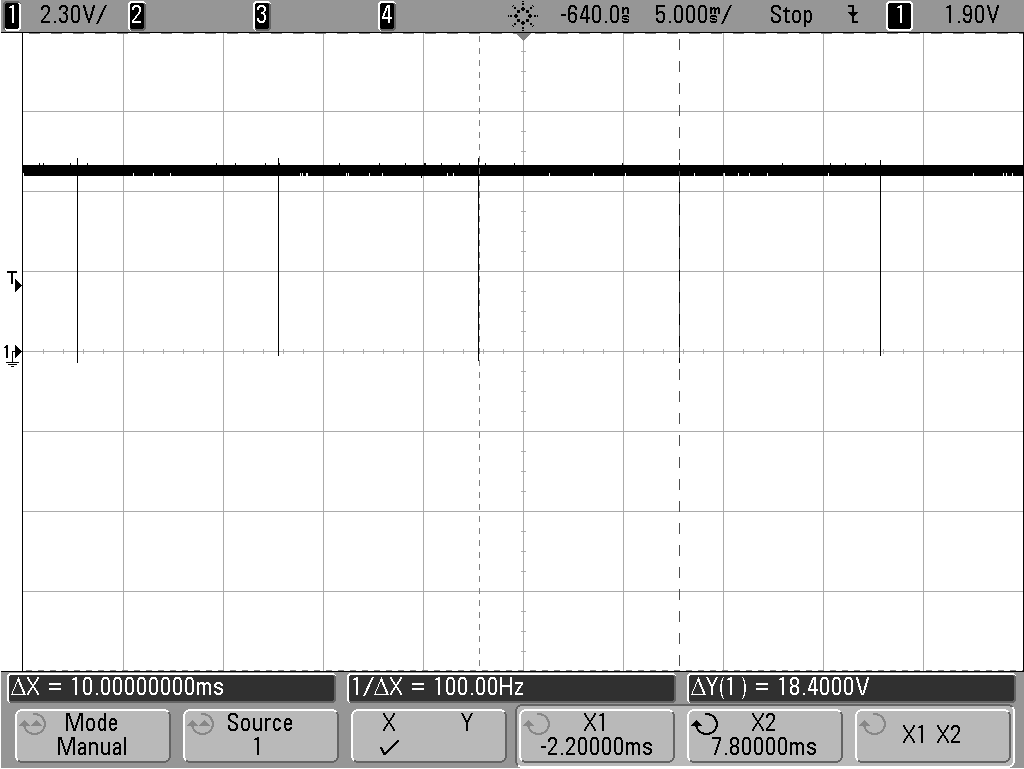
\includegraphics[scale=0.25]{ejercicio3/imagenes/riple.png}
%\caption{Respuesta a las transiciones mostradas} \label{3_fig2}
%\end{center}
%\end{figure}

\begin{figure}[H]
\begin{center}
  \begin{minipage}[b]{0.4\textwidth}
  	\begin{center}
  		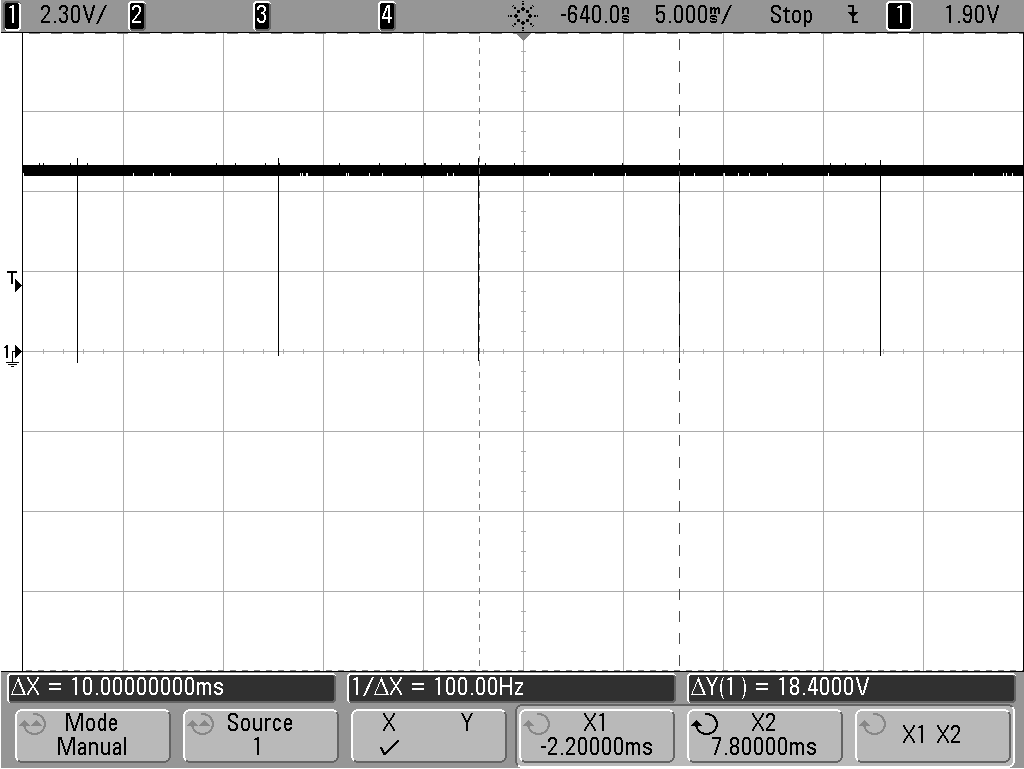
\includegraphics[scale=0.25]{ejercicio3/imagenes/riple.png}
  	\end{center}
  \caption{Respuesta a las transiciones mostradas} 
  \label{3_fig4}
  \end{minipage}
  \begin{minipage}[b]{0.4\textwidth}
    \begin{center}
  		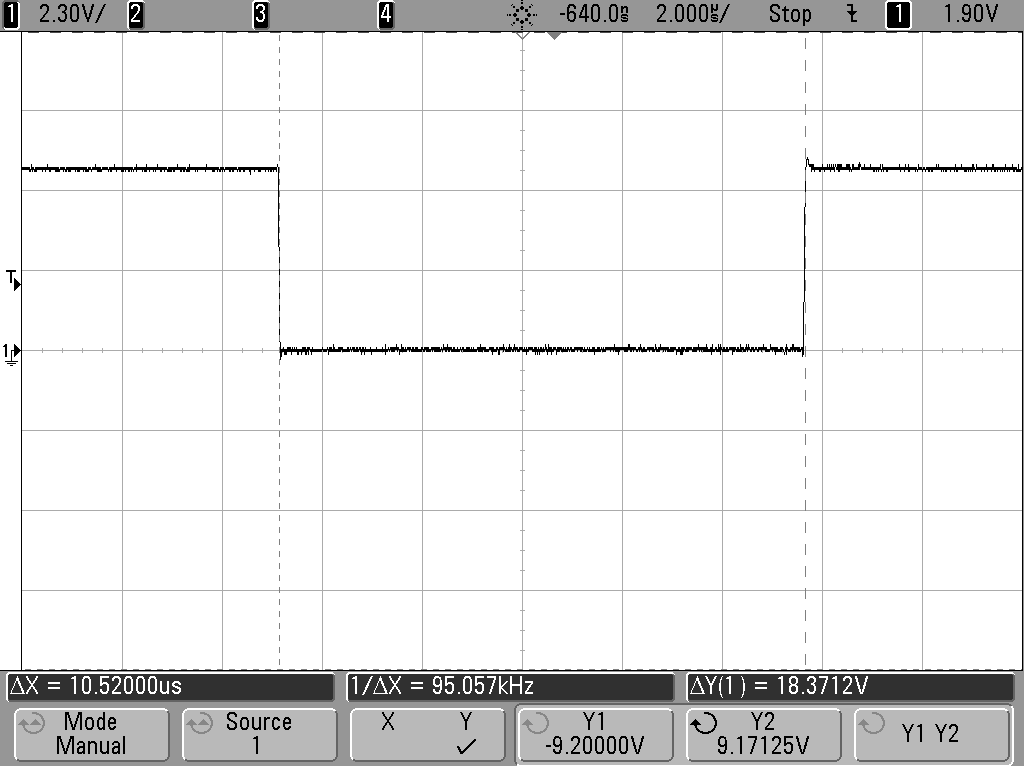
\includegraphics[scale=0.25]{ejercicio3/imagenes/tdown.png}
	\end{center}
  \caption{Ancho del pulso producido a la salida} 
  \label{3_fig5}
 \end{minipage}
\end{center}
\end{figure}

En la Figura \ref{3_fig5} se muestra una vista ampliada del pulso negativo que se mostró en la Figura \ref{3_fig4}. El ancho del pulso es de 10$\mu$seg, tiempo considerablemente largo como para producir cambios inesperados en circuitos posteriores, como ya se explicó.

%\begin{figure}[H]
%\begin{center}
%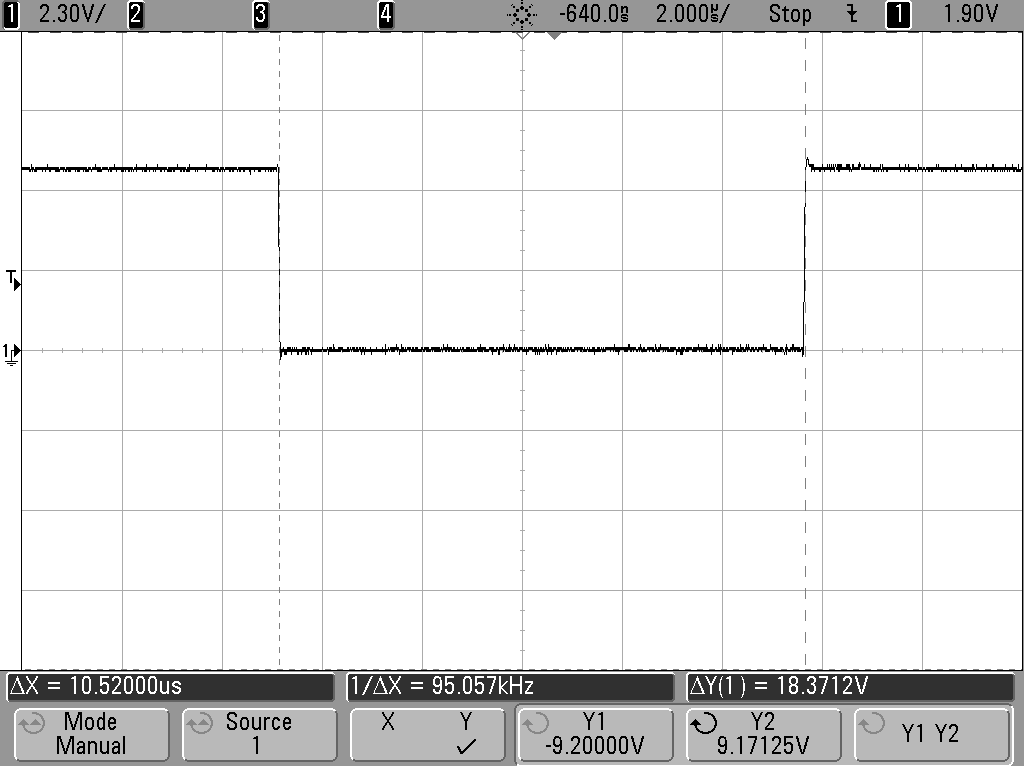
\includegraphics[scale=0.25]{ejercicio3/imagenes/tdown.png}
%\caption{Ancho del pulso producido a la salida} \label{3_fig3}
%\end{center}
%\end{figure}



